\section{Methodology and Frameworks}
\label{sec:methodology}

\subsection{CLEVR framework}
The basis for my datasets is the Visual Question Answering (VQA) framework CLEVR \citep{Johnson2017a}.
This framework provides code to generate configurable VQA datasets that are split in two parts: a collection of images, and a set of questions and answers that refer to and describe each image.
Many of the existing VQA datasets come with two problems.
First, they include many biases, such as biases in the base images and biases in the linguistic properties of the questions and answers.
A relatively high number of images of dogs in a dataset, might for instance bias a classifier model towards classifying dogs most of the time.
On the other hand, repeating patterns in the questions and answers might also be exploited by a model, without extracting the needed information from the image.
For these reasons the CLEVR framework aims to reduce the biases as much as possible in both images and questions and answers as well as precisely control the remaining biases to explore their limits.
% SD: Rather, being an artificial dataset, it allows us to precisely control the bias and therefore explore its limits.
% DK: (added; done)
Secondly, datasets may come with only a limited amount of annotations and information about the state in an image.
The CLEVR dataset uses artificially rendered 3D-scenes.
By doing so, all information about for instance the location of objects or their relations to each other can be later used in training models or analyzing their results.
Furthermore, it allows making predictions about the effects of varying contexts and information present in the scene.
% SD: We know the ground truth function that generated the scenes and hence we can also make predictions about different effects of contexts.
% DK: (added; done)

For this thesis, the CLEVR framework will be extended to have more control over the generation of the images.
With this extension, several datasets are created.
The extensions are described in Chapter \ref{sec:creation-dataset}.
Hereby, only the images and their ground truth properties are interesting for the present study of referring expressions.
% SD: We will use the code to generate a new dataset of scenes and descriptions with the properties we want to study.
% SD: You are not just taking their dataset but you are taking the framework and you are applying it on a new task, to generate a new dataset(s) with carefully controlled properties. The CLEVR framework is suitable for this because…
% DK: made clearer, what is done in the thesis, and what described in which chapter (done)
The questions and answers won't be used.
In the following section the image generation of the original CLEVR framework is described.
The visual part contains images of 3D-generated scenes depicting different kinds of simple objects.
Each of these objects is made up of a different combination of attributes, such as \emph{shape}, \emph{color}, \emph{size} and \emph{material}.
The possible values of these attributes are listed in Table \ref{tab:clevr-attributes}.
% SD: Reference to GitHub, also perhaps in the following text when you describe your own code, it would be good to include a reference to the code as you go along.
% DK: this only describes the original framework, my extension is in the next chapter with reference (done)
Three to ten objects are placed in random locations into the scene and assigned with random attributes.
To enhance realism and reduce ambiguity, objects are placed in a way so that they do not intersect and have a certain distance from each other.
Furthermore, it is made sure that every object is almost completely visible.
The positions of the light and the camera are slightly jittered for each image to add noise and reduce recurring patterns.
Since the objects are part of 3D scenes, they may look different in each image, because of different lighting and shadows, distances to the camera and rotations.
This noise approximates the real world and natural environment, and makes it harder for models to learn compared to relatively noise-free projections on a 2D plane.
Figure \ref{fig:clevr-example} shows an example of a generated image in the CLEVR dataset.

\begin{table}[ht]
    \centering
    \begin{tabular}{cccc}
        \toprule
        \textbf{ shape } & \textbf{ color } & \textbf{ size } & \textbf{ material } \\
        cube             & gray             & small           & rubber              \\
        sphere           & red              & large           & metal               \\
        cylinder         & blue                                                     \\
                         & green                                                    \\
                         & brown                                                    \\
                         & purple                                                   \\
                         & cyan                                                     \\
                         & yellow                                                   \\
        \bottomrule
    \end{tabular}
    \caption{Attributes of objects in the CLEVR dataset}
    \label{tab:clevr-attributes}
\end{table}

\begin{figure}[ht]
    \centering
    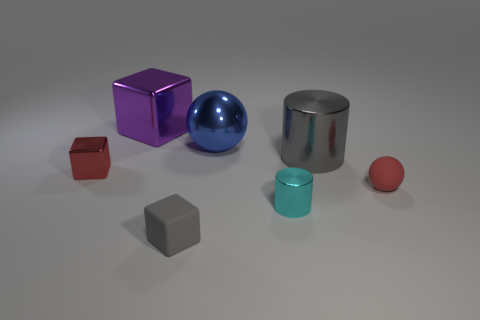
\includegraphics[width=.8\linewidth]{figures/CLEVR_example.png}
    \caption{Example of a generated image in the CLEVR dataset}
    \label{fig:clevr-example}
    % SD: Give also example of ground truth features that were used to generate this, i.e. objects and attributes.
    % DK: TODO
\end{figure}

Furthermore, the dataset contains information about each scene.
This includes all selected attributes for each object as well as the exact position of the centers of all the objects, both 3D-coordinates in the 3D scene and 2D-coordinates in the final rendered image.
In addition, simple spatial relations (in front of, behind, left, right) between the objects are calculated and stored.
% SD: For this, functions from the existing code are used, right?
% DK: exactly. Here, it is only described, what is part of the original CLEVR dataset (done)
These are simply based on the 3D-coordinates of the objects in relation to the position of the camera.

\subsection{Feature extractors}
\label{sec:feature-extractors}
In computer vision tasks, machines need to analyze images and extract information from them.
To do this, machines often rely on feature extractors.
Features are important parts or patterns in an image, which can have different levels of abstractions.
They can for example be low-level features, as geometric information about lines and edges in an image, or also very abstract information about whole objects.
Traditional approaches involve extracting key points and descriptors from an image and using them to represent the image \citep{Harris1988,Lowe1999,Bay2006}.
More recently, convolutional neural networks (CNN) became popular due to their ability to learn complex features automatically from raw image data.
These are also used in this thesis as a first layer to extract important information from the image. Hereby, two different architectures are tested.

First, we use the VGG19 \citep{Simonyan2015} which is an architecture based on many convolutional layers.
Using 16 to 19 convolutional layers with small convolution filters helps the model to solve localization and classification tasks on the training dataset, but also enables it to generalize onto other datasets.
After the convolutional layers, the data is passed first through an average pooling layer which outputs 512\times7\times7 dimensions.
Next follow three linear layers with \emph{ReLU} non-linearities in between.
After flattening the input, these classification layers output 4069, 4069 and 1000 dimensions respectively.

Secondly, we include the ResNet-101 \citep{He2016}.
This architecture tries to overcome the degradation of very deep networks, where the accuracy rapidly drops after it gets saturated.
This is done using residual blocks.
A residual block consists of two or three convolutional layers and a residual connection, also known as a shortcut connection.
The residual connection allows the input to be added directly to the output of the block, allowing the network to learn the residual function with respect to the input.
This approach enables the network to better preserve information from earlier layers and avoid the problem of information loss that can occur in very deep networks.
There are four blocks that output 256\times56\times56, 512\times28\times28, 1024\times14\times14 and 2048\times1\times1 dimensions.
A following average pooling layer outputs 2048\times1\times1 dimensions as well.
The final linear layer reduces the flattened data to 1000 dimensions, corresponding to the ImageNet classes.

Both architectures are available pretrained on an image classification task on the ImageNet dataset \citep{Deng2009}.
In this thesis, the implementations and weights available for PyTorch are used.\footnote{\href{https://pytorch.org/hub/pytorch\_vision\_resnet/}{https://pytorch.org/hub/pytorch\_vision\_resnet/}}\textsuperscript{,}\footnote{\href{https://pytorch.org/hub/pytorch\_vision\_vgg/}{https://pytorch.org/hub/pytorch\_vision\_vgg/}}
In both cases, images that should be passed through the feature extractors need to have the same structure and shape as the images that were used in the pretraining.
Hence, all images passed to them in the experiments in this thesis are preprocessed in the following way.
As described in \citep{He2016,Simonyan2015}, the images are resized to 256 pixels for the shorter side, then cropped around the center to a square of 224\times224 pixels.
Finally, the RGB channels are normalized, by subtracting the means (0,485; 0,456; 0,406) and dividing the result by the standard deviation (0,229; 0,224; 0,225) for each channel respectively.

Since the task in this research is very different from a classification, it likely learned representations that are not directly transferrable to other tasks.
The pretrained knowledge in both models might not be directly transferrable to new tasks as studied by \citet{Yosinski2014}.
In this thesis, the task differs for multiple reasons.
First, the used images for the pretraining and the present study are part of a different domain.
Even though images of the CLEVR framework are generated to resemble the real world, they still only include abstract geometric objects while ImageNet contains real photos of persons, animals and objects.
Furthermore, the original task for the pretraining is a classification task, whilst this thesis is interested in generating and understanding referring expressions.
% SD: What are the differences? Mainly in the domain of objects and scenes. What data are VGG19 and ResNet trained on?
% DK: (added; done)
For this reason, multiple different adaptions of these architectures are compared.
Table \ref{tab:feature-extractor-archs} lists the different adaptions for both VGG19 and ResNet-101 that will be used in this research.
In the later chapters, it will be referred to these adaptions using the name in the table.

\begin{table}[ht]
    \centering
    \begin{tabular}{rlc}
        \toprule
                            & \textbf{description}                                            & \textbf{ output dimensions } \\\midrule
        \textbf{VGG-0}      & contains only the convolutional layers                          & 512 \times\ 7 \times\ 7      \\
        \textbf{VGG-avg}    & contains an additional average pooling layer                    & 512 \times\ 7 \times\ 7      \\
        \textbf{VGG-cls1}   & \makecell[cl]{contains an additional one classification layer,                                 \\ including its non-linearity} & 4069                         \\
        \textbf{VGG-cls2}   & \makecell[cl]{contains another additional classification layer,                                \\ including its non-linearity} & 4069                         \\
        \textbf{VGG-cls3}   & the original VGG19 architecture                                 & 1000                         \\\midrule
        \textbf{ResNet-1}   & contains one residual block                                     & 256 \times\ 56 \times\ 56    \\
        \textbf{ResNet-2}   & contains two residual blocks                                    & 512 \times\ 28 \times\ 28    \\
        \textbf{ResNet-3}   & contains three residual blocks                                  & 1024 \times\ 14 \times\ 14   \\
        \textbf{ResNet-4}   & contains four residual blocks                                   & 2048 \times\ 1 \times\ 1     \\
        \textbf{ResNet-avg} & contains an additional average pooling layer                    & 2048 \times\ 1 \times\ 1     \\
        \textbf{ResNet-cls} & the original ResNet-101 architecture                            & 1000                         \\
        \bottomrule
    \end{tabular}
    \caption{Different adaptions of VGG19 and ResNet-101 used in this research}
    \label{tab:feature-extractor-archs}
\end{table}

% Furthermore, we experimented with both the pretrained models as well as with the architectures trained from scratch with a random initialization for the weights.
% This reason for this was to test if the success of an experiment was actually making use of the pretrained knowledge incorporated in the models.
% SD: Link to the discussion on what datasets the systems are trained on.
% If that was not the case, the agents were likely not using image features, but instead relying on some other underlying patterns to solve the task.
% Basically, this approach works as an indicator to determine the actual success of the agents aside from measures as the accuracy or precision.
% SD: This is interestingly more complex and deserves much longer discussion. Pre-trained knowledge may be unhelpful if it is very different from the new domain. Hence, at some point training from scratch may be more successful. 
% SD: What is success? Learning may take longer but then after some time the performance is better than with pre-training. 
% SD: Since agents are free to invent new language it is not clear whether this will be align with the human language that influenced pre-training the visual models, hence there is both effect of domain and language here. 
% SD: We should make these questions part of a discussion, particularly if we are comparing the effects of pre-training vs training from scratch in the experiments.
% DK: learning from scratch not part of the thesis anymore, since not the focus and much more complex (done)

\subsection{Image processing}
\label{sec:image-processing}
In the experiments different agent architectures are compared.
To make these architectures comparable, the agents' models are composed of submodules that solve a specific subtask.
Submodules can for example be image encoder modules or text parsing modules.
Hereby, different ways of solving the subtask are manifested in multiple exchangeable submodules.
For instance, one image encoder module uses CNNs while another image encoder module uses a traditional approach.
These can simply be exchanged in an agent's model without needing to adapt the whole agent.
Consequently, the experiments stay comparable, since the differences are only added or removed submodules.

The feature extractors described in section \ref{sec:feature-extractors} are not enough to be solely used to encode the images used in this thesis.
Even though final layers that contain very task and domain specific knowledge can be removed, the previous layers still don't contain any information about the new domain and task.
For this reason they need to be extended with further layers that are not frozen and can learn and store information about the new domain by connecting the pretrained general knowledge with the specific task.
These additional layers on top of the feature extractors that make up the \emph{image encoder} submodule, however, are always trained from scratch for each of the experiments and tasks.
In this thesis, only this submodule is used to encode images for all the conducted experiments.

\citet{Johnson2017} describe an architecture that was used for training baseline models on the CLEVR dataset.
This architecture will be used as the submodule.
Hereby, the image is first passed through a frozen feature extractor.
Two convolutional networks with subsequent \emph{ReLU} non-linearities condense the important information from the output of the feature extractor.
The convolutional layers reduce the channels to 128 channels, using a kernel size of 3 and a stride and padding of 1.
Afterwards, a 2-dimensional max pooling is applied with a kernel size and stride of 2.
Finally, the resulting matrix is flattened and passed through a linear layer to reduce it to an encoding size.
This vector represents the encoded image with its extracted features.
Table \ref{tab:image_encoder} shows the layers and their output dimensions when using ResNet-3 as the feature extractor and an image embedding size $e_i$.

\begin{table}[ht]
    \centering
    \begin{tabular}{ccc}
        \toprule
          & \textbf{layer}                      & \textbf{output dimensions} \\\midrule
          & Input image                         & 3 \times\ 224 \times\ 224  \\
        1 & ResNet-3                            & 1024 \times\ 14 \times\ 14 \\
        2 & Conv(3 \times\ 3, \rightarrow\ 128) & 128 \times\ 14 \times\ 14  \\
        3 & ReLU                                & 128 \times\ 14 \times\ 14  \\
        4 & Conv(3 \times\ 3, \rightarrow\ 128) & 128 \times\ 14 \times\ 14  \\
        5 & ReLU                                & 128 \times\ 14 \times\ 14  \\
        6 & MaxPool(2 \times\ 2, stride 2)      & 128 \times\ 7 \times\ 7    \\
        7 & Flatten                             & 6272                       \\
        8 & Linear Layer(\rightarrow\ $e_i$)    & $e_i$                      \\
        \bottomrule
    \end{tabular}
    \caption{Image encoder with ResNet-3 and an image embedding size $e_i$}
    \label{tab:image_encoder}
\end{table}

In some experiments, the focus of the model should be pointed to certain regions in the image.
This is done by providing the model additionally to the original image of the scene with a masked version of the scene.
In particular, the masked version only contains black and white regions.
All pixels in the relevant region are white, while all remaining pixels outside this region are black.
This is expected to help the model to learn which are the important parts in the original image.
However, a challenge lies in combining both original image and masked image.
When extracting features from an image using the previously described submodule, the output of the final linear layer doesn't directly correspond to pixels and regions in the image, but only contains the important extracted features sequentially.
In other words it looses the 2D geometrical structure of the image.
The model will have problems to align these extracted features with the masked image, still having the 2D geometrical structure.

\begin{figure}[ht]
    \centering
    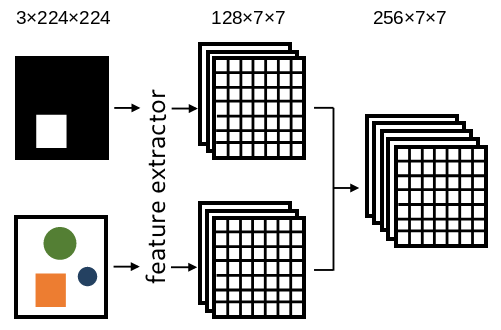
\includegraphics[width=.48\linewidth]{figures/masked_image_combination.png}
    \caption{Combination of the original image and its masked version}
    \label{fig:masked-combination}
\end{figure}

For that reason, another submodule for masked images is used, the \emph{masked image encoder}.
In this submodule, the original image and the masked image are combined at an earlier stage, when both have the same structure (see Figure \ref{fig:masked-combination}).
In particular, both images are processed in exactly the same way, by passing it through a feature extractor and then through the above described extending layers until layer 6, the max pool layer.
Even though  the masked image doesn't contain similar features to the images the feature extractors are pretrained on, this method still provided better results in the experiments.
After this, the images are concatenated along the channels, which results in a matrix with the dimensions 256\times7\times7 (still including the geometrical structure with 7\times7 grids).
Finally, this matrix is flattened and reduced to the image embedding size $e_i$.
Doing this, the model can directly align a region in the original image with a region in the masked image.

\subsection{EGG framework}
\label{sec:methodology:egg}
The goal of this thesis is to run and compare different setups of language games systematically.
To do this, all experiments rely on the \emph{\textbf{E}mergence of lan\textbf{G}uage in \textbf{G}ames} (EGG) framework \citep{Kharitonov2019} which is implemented in PyTorch.
% SD: What is the framework? We saw that language games can be implemented very differently, with robots, as code, etc. it is a neural model.
% DK: (added; done)
This framework allows the implementation of language games in code, where agents are neural models that communicate with each other.
It consists of a heavily configurable core that controls the generating and parsing of the message, the calculation of the loss and the rules, for how the weights of all neural models are trained.
% SD: You frequently start discussion by referring to quite specific concepts straight away in a very concise way, e.g. Gumbel Softmax, Reinforce, without defining them but then an explanation comes later in the text. The problem with this a reader would wonder what they are and would look for explanation. It is best to have a very general introduction, e.g. we will test two optimisation functions and then introduce them and explain them in one go later.
% DK: (rephrased; done)
The configuration includes for example:
\begin{itemize}[noitemsep,topsep=0pt]
    \item a choice between single symbol and sequence messages with varying RNNs,
    \item an easy switch between different loss functions,
    \item or a choice between two optimization functions (Gumbel-Softmax relaxation and REINFORCE algorithms) to learn neural models containing discrete symbols.
\end{itemize}
% SD: More detailed description of all these. Readers will not be familiar with Gumbel-Softmax for example.
% DK: (rephrased; done)
Furthermore, runs of games can be saved to analyze the used messages of the agents and how they vary over the duration of the learning.

\begin{figure}[ht]
    \centering
    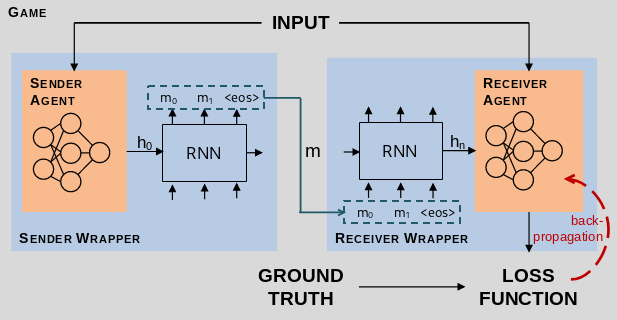
\includegraphics[width=.8\linewidth]{figures/egg_framework.png}
    \caption{The EGG framework is made up of three levels: the game (gray), the wrappers (blue) and the agents (orange)}
    \label{fig:egg-framework}
\end{figure}

The EGG framework is set up in three levels, shown in .
Part of the lowest level are the \emph{agents} themselves.
The agents are neural models that need to be implemented from scratch and define how the agents process their input and in case of the receiver combine it with the message.
The second level consists of \emph{wrappers} that take care of generating and parsing the message.
The sender wrapper uses the output of the sender agent, to produce a message.
The receiver wrapper on the other hand parses the message received by the sender and passes the result as an additional input to the receiver agent.
The third level, the \emph{game}, links all described parts together.
It provides the agents with the input and passes the message from the sender to the receiver.
Furthermore, it uses the output of the receiver and calculates the loss, which is then the basis for the adaption of the weights for both wrappers and agents.
% SD: Include a diagram?
% DK: done

For the language games which are run in this thesis, the sender will always produce a sequence of symbols as a message, which the receiver will parse.
Gumbel-Softmax relaxation is applied to produce discrete symbols.
This is done in the default method of the EGG framework using two LSTMs, an encoder LSTM in the sender wrapper and a decoder LSTM in the receiver wrapper.
The output of the sender agent is used as the initial hidden state for the encoder LSTM.
% SD: This sounds like details of your implementation and should come later. Here, we would only need a general description of the EGG framework. Also for this text later, it would be good to have a diagram of all these steps and examples what these games actually are.
% DK: this is actually the default implementation in EGG in therefore described here (TODO, diagram)
This LSTM is then producing symbols until it generates an end-of-sequence symbol.
This sequence is then passed to the receiver wrapper with its decoder LSTM.
Its hidden state is initialized randomly.
The received message sequence is processed symbol by symbol.
After each time, a symbol is processed by the LSTM, the resulting new hidden state is passed to the receiver agent as the parsed message.
The receiver agent is combining it with its representation of the image input and is predicting an output.
In other words the receiver agent produces as many outputs as symbols are present in the message.
The \emph{game} is then calculating a loss for each of these outputs separately.
These losses are summed up to a total loss that is used to adapt the weights in both agents as well as in both LSTMs.

\subsection{Optimization in language games}
\label{sec:methodology:optimization}
Training agents in a language game is not a straight forward task.
In this thesis, the agents share a common goal, in particular optimizing the predictions of the receiver.
The loss function of the whole game can therefore be defined as the loss of the receiver's predictions given its input and the sender's message.
By this, the receiver can be trained relatively easily by backpropagating the game's loss through all layers in the model of the receiver.
A problem however arises when passing on the loss to the sender.
The generation of the message involves sampling from a categorical distribution and is therefore not differentiable.
Consequently, the gradients of the loss function can't be estimated with standard backpropagation methods for the sender.
To solve this problem two dominant methods are currently used: REINFORCE algorithms \citep{Williams1992} and Gumbel-Softmax relaxation \citep{Jang2017}.

The traditional approach to solve problems with a discrete channel formulates the problem as a reinforcement learning task and relies on the REINFORCE algorithms.
In reinforcement learning, the neural models are trained to optimize their policy given a reward.
Given for example the referential game, described in \citep{Lazaridou2017}, where the sender is presented with two images and needs to communicate the target image to the receiver.
The receiver is shown the same images and is tasked to point to the correct target image given the sender's message.
The sender model and receiver model are following a policy with parameters $\theta$ respectively.
The policy of the sender can be defined as $s(\theta_S(i_L,i_R,t)) \in V$ with $\theta_s$ being the parameters of the senders neural model, $i_L$ and $i_R$ the presented images, $t$ the target image and $V$ the vocabulary.
The receiver's policy is dependent on the message by the sender and therefore directly dependent on the sender's policy and can be defined like this: $r(i_L,i_R,s(\theta_S(i_L,i_R,t))) \in \{L,R\}$.
The reward is given if the receiver's policy successfully produced the target image:
\begin{equation}
    R =
    \begin{cases}
        1, & \text{iff } r(i_L,i_R,s(\theta_S(i_L,i_R,t))) = t \\
        0, & \text{otherwise}
    \end{cases}
\end{equation}

The task for the agents to learn is to maximize the reward function $R$ across all possible rewards (dependent on receiver's policy and target image) $\mathbb{E}_{\tilde{r}}[R(\tilde{r})]$.
The problem hereby is that not all possible rewards are known.
Without training, it can't be determined if a certain configuration of the agents, the policy, yields the correct target image.
The rewards are in fact the outcome of the training.
To solve this, Monte Carlo sampling is used to approximate the expected value $\mathbb{E}$.
Monte Carlo sampling works on the fact that the mean of all drawn samples from an unknown probability distribution approximates its expected value.
The more samples are drawn, the better the approximation.
Using the approximation, the function becomes differentiable and can be used to calculate the gradients to update the policies.
In this case, the approximation is based on the already determined rewards, in other words on the already played games.
Early games are more or less trial and error, because the approximation is very bad.
Only when many games are played, the approximation becomes better and the models can be updated properly.
This however also means that the training can take very long until the models start to converge, and it suffers from high variance.

For this reason, more recently Gumbel-Softmax relaxation is used to represent the discrete message.
Basically, this method is a way to turn a discrete categorical distribution into a continuous distribution that can be differentiated.
By doing this, sender and receiver are completely differentiable and act as whole deep neural model where the loss can be backpropagated with standard methods.
In particular the problem lies in sampling from the categorical distribution $C$  over $|V|$ symbols, which can't be differentiated.
Therefore, the method applies a reparameterization trick: random samples are instead drawn from the Gumbel distribution $G$ (Equation \ref{eq:gumbel-sample}) and summed with the logarithmic probabilities of each symbol (Equation \ref{eq:reparameterization}).
\begin{align}
    g   & = -log(-log(u))  & \text{ with }u\sim Uniform(0,1) \label{eq:gumbel-sample} \\
    s_k & = log(c_k) + g_k & \text{ for }k = 1,...,|V| \label{eq:reparameterization}
\end{align}

To determine the symbol to use, usually the $argmax$ function would be applied on the resulting vector $s$.
However, this function is again undifferentiable and is therefore approximated using the $softmax$ function:
\begin{equation}
    y_k = \frac{exp(s_k / \tau)}{\sum_{i=1}^{|V|}{exp(s_i / \tau)}}
\end{equation}
The temperature $\tau$ of the $softmax$ function determines how well it approximates the $argmax$ function.
For $\tau \to 0$, the samples from the Gumbel-Softmax distribution are identical with the categorical distribution while for $\tau \to \infty$ the Gumbel-Softmax distribution becomes uniform.

The Gumbel-Softmax method offers stable gradient estimates and can be more efficient than the traditional REINFORCE algorithm, especially when dealing with large action spaces.
This also applies to language games, where \citet{Havrylov2017} demonstrated that Gumbel-Softmax relaxation is more effective.
For that reason, the experiments in this thesis utilize Gumbel-Softmax relaxation.
% SD: This is what a technical manual would say - but what does it do really? What is the difference between reinforce and Gumbel softmax in practice? In our case? Reinforce is still superior but here you make it less.
% DK: I don't think, REINFORCE is superior also in our case, since GS offers more stability in learning (see citing) (TODO, explain GS)

\subsection{Ethical considerations}
In the field of natural language processing (NLP) ethical issues often play major roles.
These can be part of the used datasets, the created models and their training as well as the application of the models.
For datasets, the role data privacy is increasing with the necessity of larger amounts of data \citep{Klymenko2022}.
Furthermore, datasets often contain biases, based for instance on the authors of the collected natural language texts. Often they also contain biases such as overrepresentations and underrepresentations.
Even though some of these biases are inherent to the data and not necessarily negative, much research is indicating that undetected and unaddressed biases in datasets might lead to negative consequences \citep{Shah2020,Field2021,Bender2021}.
Training neural models can also lead to environmental issues, as large models need to process huge amounts of data and require a lot of energy \citep{Bender2021}.
Finally, the application of trained models can create harm.
This applies for example to easy accessible large language model (LLMs) that can be used to create information hazard \citep{Weidinger2022}.

The research in this thesis tries to reduce these risks.
Looking at the datasets that are used in this thesis, all data is created artificially and contains therefore no personal information.
Even further, the aim of the creation of these datasets is to reduce and study the remaining biases.
% SD: to study biases
% DK: (rephrased; done)
It doesn't include any social information, but on the other hand consists only of abstract scenes.
The choice of which attributes the objects are made up is inherently biased towards human cognition, but doesn't have a social impact.
The models and agents are therefore trained, by including as few human biases as possible.

Looking at the environmental issues, the models used in this thesis consist of only few trained layers and the training is therefore short and doesn't require much energy.
Larger models as the feature extractors are already pretrained and add no additional consumption.

Finally, the purpose of this thesis is to analyze the results and the emerged language and draw conclusions, how emerged languages can be grounded better in the environment.
For that reason, the final models can't be used in any real world applications and produce potential harm.
On the other hand, this work can on the long run mitigate harm as it provides a study of models, how they would behave on real data.
This therefore contributes towards interpretability of AI.
% SD: The work can on the long run mitigate harm as it is provides a study of models, how they would behave on real data and therefore contributes towards interpretability of AI.
% DK: (added; done)
